\section{研究背景}

\subsection{选题意义}
\begin{frame}{选题意义}
    \begin{columns}
        \column{0.5\textwidth}
        在地理国情监测
        中, 光学遥感卫星数据多源, 可视判读性高得到广泛应用. 我国热带, 亚热带地区, 受多云多雨气候影响, 可用于生产单位的光学影像少, 无法满足我国多云多雨地区耕地保护动态需求.

        \column{0.5\textwidth}
        
        \begin{figure}
            \centering
            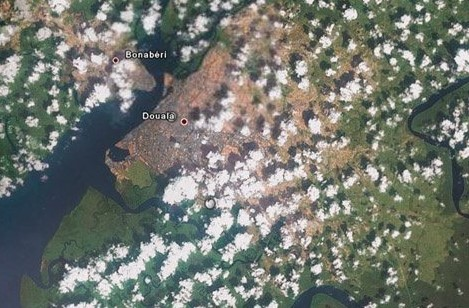
\includegraphics[width=\textwidth]{pic/chap0101.jpg}
            \caption{云雾覆盖光学影像}
            \label{fig:0101}
        \end{figure}
    \end{columns}
\end{frame}

\begin{frame}{选题意义}
    \begin{columns}
        \column{0.5\textwidth}
        \begin{figure}
            \centering
            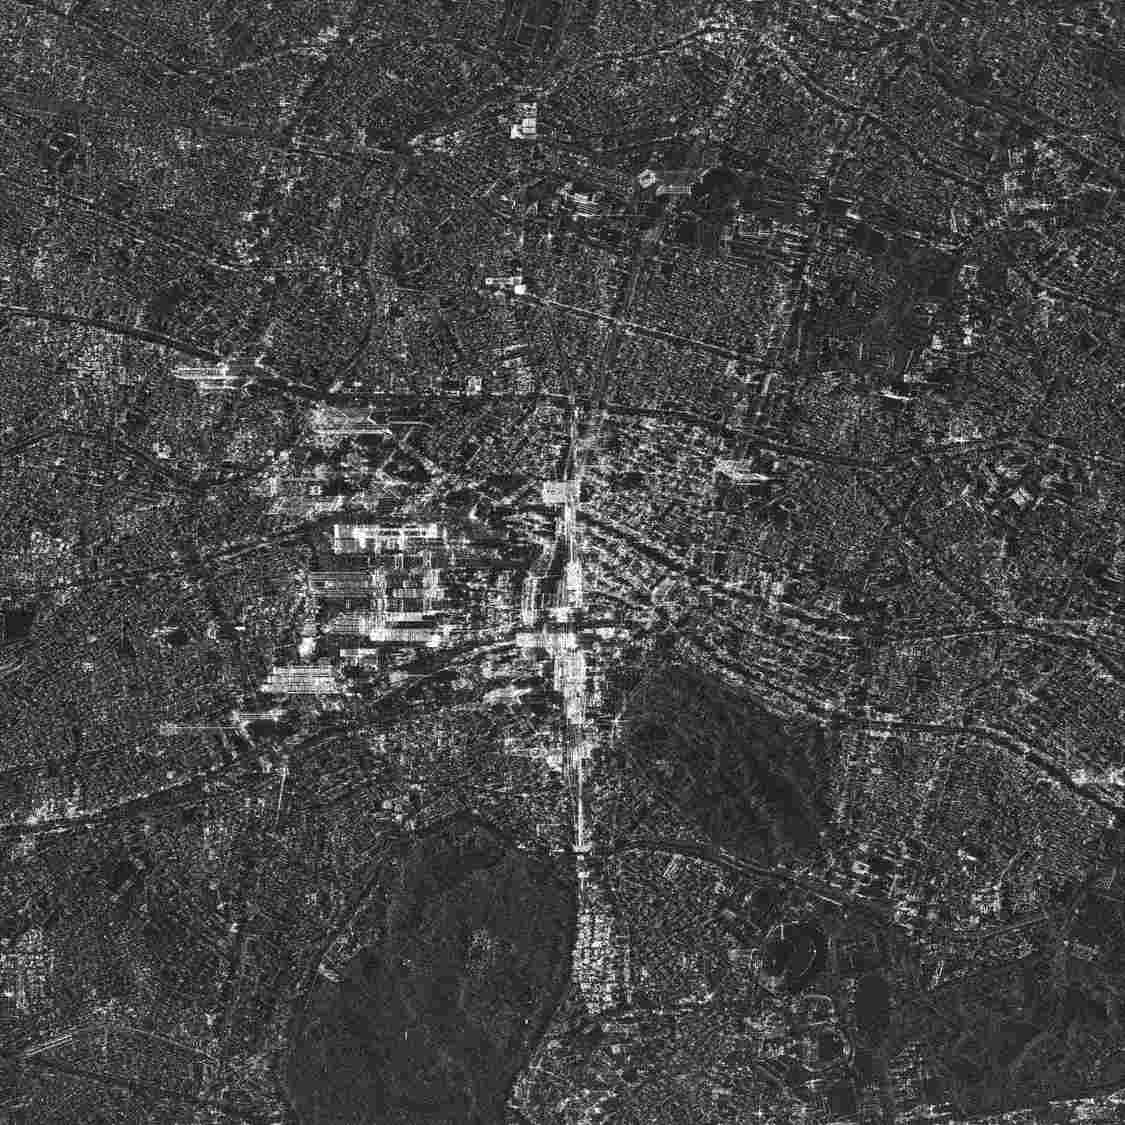
\includegraphics[width=\textwidth]{pic/chap0102.jpg}
            \caption{SAR影像}
            \label{fig:0102}
        \end{figure}

        \column{0.5\textwidth}
        合成孔径雷达虽可穿云透雨, 但因成像机理不同, 可读性远低于光学遥感影像. 以广东为例, 国内发射高分辨率SAR卫星无法全覆盖我国多云雨地区, 而国外米级亚米级卫星价格昂贵, 生产单位无法接受. 中分辨率SAR卫星影像, 如哨兵一号, 虽开源, 但不能满足我国地理国情监测需求.
    \end{columns}
\end{frame}

\begin{frame}{选题意义}
    \begin{columns}
        \column{0.5\textwidth}
        近年来, 随着深度学习迅速发展, 图像生成技术成功应用到许多领域. 因此, 利用国外免费中分辨率SAR卫星影像, 使用图像翻译和超分技术, 重构光学高分辨率影像, 在生产单位不增加数据购买成本的情况下, 解决我国热带亚热带光学卫星缺失问题, 有重要研究意义.
        
        \column{0.5\textwidth}
        \begin{figure}
            \centering
            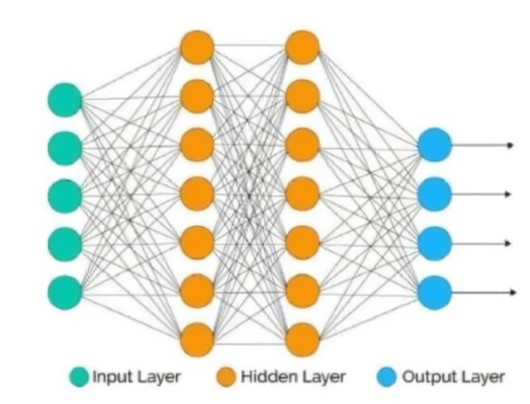
\includegraphics[width=\textwidth]{pic/chap0103.jpg}
            \label{fig:0103}
        \end{figure}
    \end{columns}
    


\end{frame}

\subsection{文献综述}

\begin{frame}{图像生成}
    \begin{columns}
        \column{0.4\textwidth}
        \begin{figure}
            \centering
            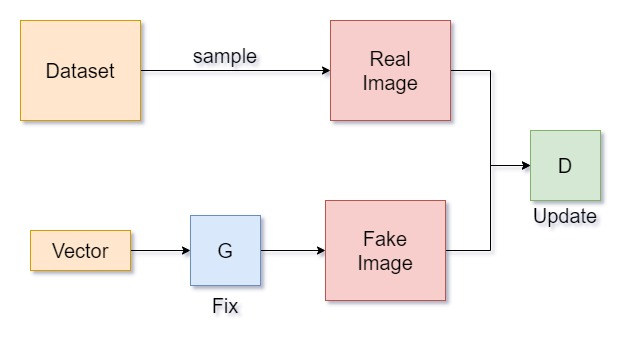
\includegraphics[width=\textwidth]{pic/chap0104.jpg}
            \label{fig:0104}
        \end{figure}

        \column{0.6\textwidth}
        图像生成: 对自然图像的分布进行建模及生成图像
        \begin{itemize}
            \item 玻尔兹曼机, 自编码器, 变分自编码器(VAE)
            \item 生成对抗网络(GAN)
        \end{itemize}

        针对原始GAN的问题, 有以下:
        \begin{itemize}
            \item 稳定性: WGAN, WGAN-GP, LSGAN等
            \item 图像质量: LapGAN, ProGAN, SAGAN, BigGAN
        \end{itemize}
    \end{columns}
    % 学术界对图像生成进行了广泛探索, 许多工作着重对自然图像的分布进行建模以及生成图像. 这个问题最初可由玻尔兹曼机和自编码器解决, 之后变分自编码器通过对隐变量分布进行重新参数化来提高图像生成质量和效率. 

    % 另一方面生成对抗网络(GAN)通过生成器和判别器两个网络进行极大极小训练策略从随机变量中生成图像. 原始GAN面临两个挑战, 意识训练稳定性, 二是生成高分辨率图像能力有限. 为了解决GAN稳定性问题, WGAN, WGAN-GP, LSGAN等损失函数被提出. LapGAN, ProGAN, SAGAN, BigGAN从不同方法提高了图像生成质量.
\end{frame}

\begin{frame}{图像到图像翻译}  
    \begin{columns}
        \column{0.5\textwidth}
        \begin{figure}
            \centering
            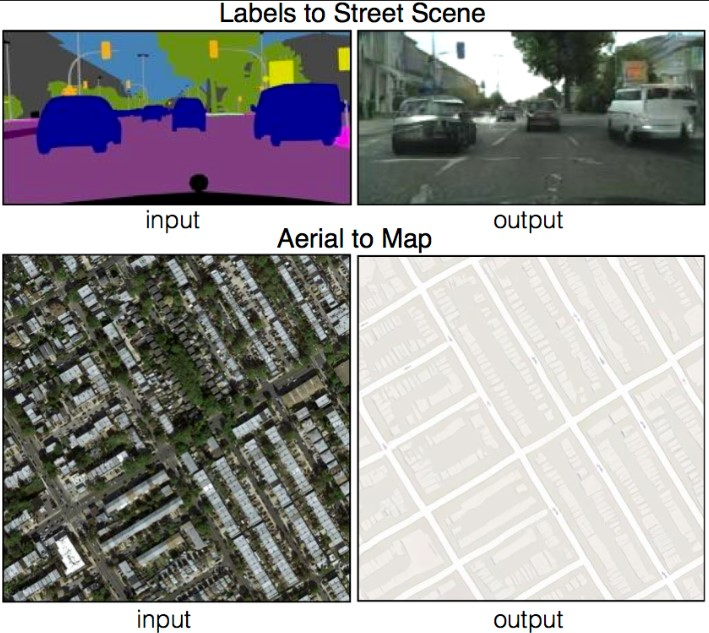
\includegraphics[width=\textwidth]{pic/chap0105.jpg}
            \caption{Pix2Pix}
            \label{fig:0105}
        \end{figure}

        \column{0.5\textwidth}
        \begin{itemize}
            \item Isola等人提出Pix2Pix, 利用对抗损失提高图像生成质量
            \item Zhu考虑到源域一对多目标域影像, 提出双射一致性学习图像到图像翻译
            \item Chen等人提出重级联细化网络(CRN), 逐步细化合成高分辨率图像
        \end{itemize}

    \end{columns}

    % 图像翻译已经成为图像生成中的热门研究领域. 由于深度学习蓬勃发展, 近年图像到图像的翻译主要集中利用CNN在一个含有成对输入输出样本的数据集上学习此类图像映射.

    % Isola等人提出通用的CGAN(Pixel2Pixel), 用于有监督图像翻译工作, 包括标签到街景, 卫星地图到平面地图等. 除了传统L1损失函数, Pix2Pix利用对抗损失提高生成质量. Pix2Pix给定一个输入只有一个输出, 考虑到源域中一个影像对应目标域多个影像, Zhu等人进一步提出双射一致性学习图像至图像翻译. Chen等人提出以重级联细化网络, 逐步细化合成高分辨率图像.
\end{frame}

\begin{frame}{图像到图像翻译}
    \begin{columns}
        \column{0.6\textwidth}
        在实际应用中, 很难为有监督图像到图像翻译收集大量成对数据. 无监督图像翻译主要学习源域和目标域之间映射.
        \begin{itemize}
            \item Dumoulin等人和Doahue等人提出无监督学习隐式变量空间和图像数据空间之间的双向映射算法
            \item Taigman等人提出域变换网络(DTN)
            \item He等人提出对偶学习机制, DualGAN, DiscoGAN, CycleGAN几乎同一时间被提出, 它们同时训练两个GAN解决不成对图像翻译问题.
        \end{itemize}

        \column{0.4\textwidth}
        \begin{figure}
            \centering
            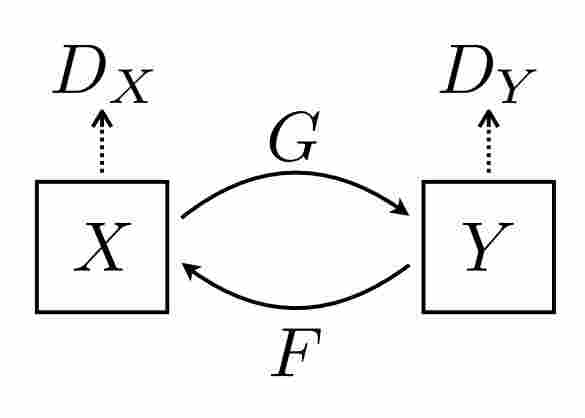
\includegraphics[width=\textwidth]{pic/chap0106.jpg}
            \caption{CycleGAN}
            \label{fig:0106}
        \end{figure}

    \end{columns}

    % 但在实际应用中, 很难为有监督图像到图像翻译收集大量成对数据, 因此无监督使用不成对的图像到图像翻译的方法受到关注. 除了学习源图像域和目标图像域之间映射, Dumoulin和Doahue等人提出无监督学习隐式变量空间和图像数据空间之间的双向映射算法. Taigman等人提出域变换网络, He等人提出对偶学习机制, DualGAN, DiscoGAN, CycleGAN几乎同一时间被提出, 它们同时训练两个GAN解决不成对图像翻译问题.
\end{frame}

\begin{frame}{图像超分}
    \begin{columns}
        \column{0.6\textwidth}
        针对单张图像的超分辨率重建主要有基于插值, 基于重建和基于学习的方法. 基于插值方法较为简单, 但不能有效恢复图像中的高频信息, 导致图像模糊; 基于重建的方法通过先验假设某一退化模型, 对模型中的退化参数进行估计, 通过求解其逆变换得到高分辨率影像. 

        \column{0.4\textwidth}
        \begin{figure}
            \centering
            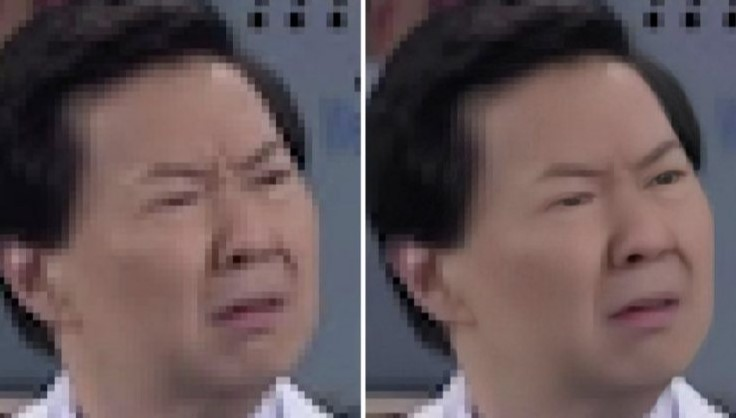
\includegraphics[width=\textwidth]{pic/chap0107.jpg}
            \caption{超分}
            \label{fig:0106}
        \end{figure}

    \end{columns}
\end{frame}

\begin{frame}{图像超分}
    

    近几年来, 深度学习在超分重建中取得显著成绩. 
    
    \begin{itemize}
        \item SRCNN首次使用CNN来解决超分问题, VDSR针对SRCNN模型结构较浅, 非线性表达能力不足提出一种深层网络.
        \item SRResNet提出使用残差模块处理超分问题. 
        \item SRGAN首先将GAN引入超分领域, 在原有GAN损失函数加Content Loss. ESRGAN将SRGAN中的BN模块用Dense Block模块代替, 提高了超分质量.
        \item KernelGAN则通过估计退化模型的方式 
        \item DDGAN, SRRESCGAN则在超分过程中引入Domain Translation的思想.
    \end{itemize}
    
       
\end{frame}
